\documentclass[10pt,final,a4paper,oneside,onecolumn]{article}

%%==========================================================================
%% Packages
%%==========================================================================
\usepackage[a4paper,left=3.5cm,right=3.5cm,top=3cm,bottom=3cm]{geometry} %% change page layout; remove for IEEE paper format
\usepackage[T1]{fontenc}                        %% output font encoding for international characters (e.g., accented)
\usepackage[cmex10]{amsmath}                    %% math typesetting; consider using the [cmex10] option
\usepackage{amssymb}                            %% special (symbol) fonts for math typesetting
\usepackage{amsthm}                             %% theorem styles
\usepackage{dsfont}                             %% double stroke roman fonts: the real numbers R: $\mathds{R}$
\usepackage{mathrsfs}                           %% formal script fonts: the Laplace transform L: $\mathscr{L}$
\usepackage[pdftex]{graphicx}                   %% graphics control; use dvips for TeXify; use pdftex for PDFTeXify
\usepackage{array}                              %% array functionality (array, tabular)
\usepackage{upgreek}                            %% upright Greek letters; add the prefix 'up', e.g. \upphi
\usepackage{stfloats}                           %% improved handling of floats
\usepackage{multirow}                           %% cells spanning multiple rows in tables
%\usepackage{subfigure}                         %% subfigures and corresponding captions (for use with IEEEconf.cls)
\usepackage{subfig}                             %% subfigures (IEEEtran.cls: set caption=false)
\usepackage{fancyhdr}                           %% page headers and footers
\usepackage[official,left]{eurosym}             %% the euro symbol; command: \euro
\usepackage{appendix}                           %% appendix layout
\usepackage{xspace}                             %% add space after macro depending on context
\usepackage{verbatim}                           %% provides the comment environment
\usepackage[dutch,USenglish]{babel}             %% language support
\usepackage{wrapfig}                            %% wrapping text around figures
\usepackage{longtable}                          %% tables spanning multiple pages
\usepackage{pgfplots}                           %% support for TikZ figures (Matlab/Python)
\pgfplotsset{compat=1.14}						%% Run in backwards compatibility mode
\usepackage[breaklinks=true,hidelinks,          %% implement hyperlinks (dvips yields minor problems with breaklinks;
bookmarksnumbered=true]{hyperref}   %% IEEEtran: set bookmarks=false)
%\usepackage[hyphenbreaks]{breakurl}            %% allow line breaks in URLs (don't use with PDFTeX)
\usepackage[final]{pdfpages}                    %% Include other pdfs
\usepackage[capitalize]{cleveref}				%% Referensing to figures, equations, etc.
\usepackage{units}								%% Appropriate behavior of units
\usepackage[utf8]{inputenc}   				 	%% utf8 support (required for biblatex)
\usepackage{csquotes}							%% Quoted texts are typeset according to rules of main language
\usepackage[style=ieee,doi=false,isbn=false,url=false,date=year,minbibnames=15,maxbibnames=15,backend=biber]{biblatex}
%\renewcommand*{\bibfont}{\footnotesize}		%% Use this for papers
\setlength{\biblabelsep}{\labelsep}
\bibliography{../../bib}

%%==========================================================================
%% Define reference stuff
%%==========================================================================
\crefname{figure}{Figure}{Figures}
\crefname{equation}{}{}

%%==========================================================================
%% Define header/title stuff
%%==========================================================================
\newcommand{\progressreportnumber}{5}
\renewcommand{\author}{Erwin de Gelder}
\renewcommand{\date}{22 February 2018}
\renewcommand{\title}{Performance assessment of automated vehicles using real-life driving scenarios}

%%==========================================================================
%% Fancy headers and footers
%%==========================================================================
\pagestyle{fancy}                                       %% set page style
\fancyhf{}                                              %% clear all header & footer fields
\fancyhead[L]{Progress report \progressreportnumber}    %% define headers (LE: left field/even pages, etc.)
\fancyhead[R]{\author, \date}                           %% similar
\fancyfoot[C]{\thepage}                                 %% define footer


\newlength\figurewidth
\newlength\figureheight

\begin{document}
	
\begin{center}
	\begin{tabular}{c}
		\title \\ \\
		\textbf{\huge Progress report \progressreportnumber} \\ \\
		\author \\ 
		\date
	\end{tabular}
\end{center}

\section{Previous meeting minutes}

\begin{itemize}
	\item The paper ``Ontology of scenario for the assessment of automated vehicles'' for the Intelligent Vehicles Symposium 2018 is almost finished. The paper has to be reviewed by Jeroen and Bart. Deadline is the 29th of January.
	\item For the graduate school, I need to obtain 45 Graduate School Credits (GSCs) that are divided into three parts of 15 GSCs:
	\begin{itemize}
		\item \emph{Research skills}: These are Learning-on-the-Job Activities, e.g., paper review, presentation, poster, paper writing. I assume that these GSCs will be automatically achieved during the PhD, so no special planning regarding this is needed.
		\item \emph{Discipline-related skills}: This relates to skills that improve knowledge related to the research. I will look if I can find some courses in Singapore.
		\item \emph{Transferable skills}: These skills will improve myself on a personal level. When I return from Singapore, I will look for useful courses.
	\end{itemize}
	\item We discussed about the report I wrote regarding the generation of test cases. A couple of remarks regarding the report:
	\begin{itemize}
		\item The problem formulation was at best very vague.
		\item Possibilities for the use of copulas should be shortly summarized.
		\item Most parts were not properly explained and notation of variables was confusing.
		\item For a similarity measure that quantifies the similarity between two profiles, it would make sense to normalize it, such that it is between $0$ and $1$.
	\end{itemize}
\end{itemize}

\section{Summary of work}

\begin{figure}
	\centering
	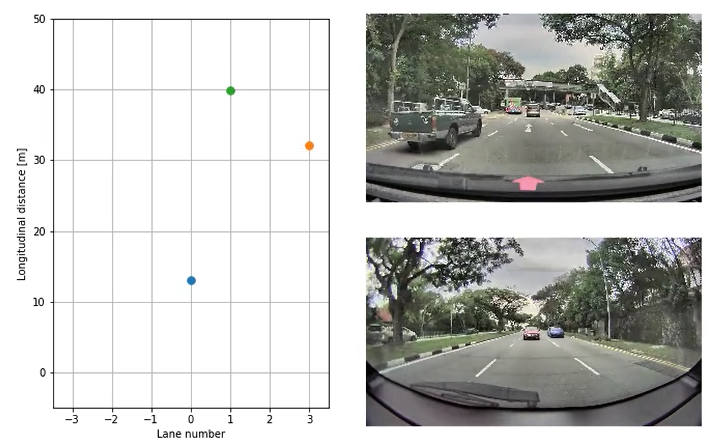
\includegraphics[width=0.8\linewidth]{bmw_example}
	\caption{Example of a frame of the data. In the left plot, the detected objects are shown (different color means different ID). On the right, the images of the front view camera (top) and rear view camera (bottom) are shown.}
	\label{fig:bmw example}
\end{figure}

\begin{itemize}
	\item I got access to a very small piece of the data acquired by BMW in Singapore. See \cref{fig:bmw example} for an example of a sample. Some observations:
	\begin{itemize}
		\item Many objects are not detected. For example, the car on the left side (see \cref{fig:bmw example}) is not detected. It seems that the field of view is very limited.
		\item The object data seems to be processed with a low pass filter with a very low bandwidth. For example, the car in front (see \cref{fig:bmw example}) already increased distance with approximately $\unit[5]{m}$, but this is only visible in the object data after few seconds.
	\end{itemize}
	\item I did some research regarding similarity measures for time series, because an appropriate similarity measure for comparing two different scenarios would be useful for at least two reasons:
	\begin{itemize}
		\item To quantify to what extent a certain set of scenario is complete, it would be useful to quantity the similarities among the scenarios. If each scenario is very different from all other scenarios, this is an indication that the set of scenarios does not reflect all possible variations. To quantify the `difference' between two scenarios, a (dis)similarity measure could be employed.
		\item To quantify how realistic a generated scenario is, it could be compared with real-world scenarios. If the generation scenario differs significantly from the real-world scenarios, it could be an indication that the generation scenario is not realistic.
	\end{itemize}
	A report is attached to this progress report\footnote{Note that the page numbers in the table of contents of the attached report are not correct, as those page numbers refer to the original report (before it was included in this progress report).} that reflects my findings.
	\item The paper for the Intelligent Vehicle Symposium (IV) 2018 is submitted. On the 31st of March we will receive a notification of acceptance. For your information, the paper is attached to this document (starting at page \pageref{ivpaper}).
\end{itemize}

\section{Future plans}

\begin{itemize}
	\item I wrote a document regarding similarity measures for time series. I want to apply one or several measures for quantifying the completeness of a set of real-world scenarios. As a start, I can use a small dataset with time series of the speed while the car is braking (approximately 3000 time series). Eventually, if we want to write a paper on this subject, we need more scenario classes, as one example is too limited.
	\item For my work in Singapore, I need to define 15 different scenarios classes and the way we want to parametrize these scenarios. Ideally, I want to show at least one real-world scenario for each scenario class.
	\item Before applying the dissimilarity measure for estimating the \emph{completeness}, I want to search for more relevant literature on this subject. Wang et al.~\cite{wang2017much} claim to be the to write a paper about \emph{completeness} with respect to naturalistic driving data, but I think there should be more relevant literature (including other applications).
\end{itemize}

\section{Questions}

\begin{itemize}
	\item I reviewed several dissimilarity measures and I see two possible candidates for further usage:
	\begin{itemize}
		\item Using custom parameters as this gives high freedom in what makes scenarios distinctive. The disadvantage is that there is not a general recipe for choosing the parameters, while the choice of the parameters highly influence the resulting dissimilarity measures.
		\item Dynamic Time Warping (DTW) looks promising, because it corrects for time shifts and this might be a useful feature. For example, consider the two scenarios in \cref{fig:early detection}. With DTW, the dissimilarity score between these two time series would be very low, because the time series $\textbf{v}_2$ will be `warped' such that it looks exactly similar to the `early detection'. In most cases, this will be useful.
	\end{itemize}
	What measure is or what measures are the most promising to continue with?
\end{itemize}

\begin{figure}
	\centering
	\setlength\figurewidth{0.7\textwidth}
	\setlength\figureheight{0.5\textwidth}
	% This file was created by matplotlib2tikz v0.6.16.
\begin{tikzpicture}

\definecolor{color0}{rgb}{0.12156862745098,0.466666666666667,0.705882352941177}
\definecolor{color1}{rgb}{1,0.498039215686275,0.0549019607843137}

\begin{axis}[
xlabel={Sample},
ylabel={Speed [m/s]},
xmin=-4.05, xmax=85.05,
ymin=-0.654, ymax=13.734,
width=\figurewidth,
height=\figureheight,
tick align=outside,
tick pos=left,
xmajorgrids,
x grid style={white!69.01960784313725!black},
ymajorgrids,
y grid style={white!69.01960784313725!black},
legend style={draw=white!80.0!black},
legend cell align={left},
legend entries={{$\textbf{v}_{2}$},{Early detection}}
]
\addlegendimage{no markers, color0}
\addlegendimage{no markers, color1}
\addplot [semithick, color0, mark=*, mark size=1, mark options={solid}, only marks]
table {%
0 13.08
1 13.0299962102895
2 12.9999910191757
3 12.9299945128149
4 12.8799917292974
5 12.8099888480973
6 12.7599611554673
7 12.6249483953104
8 12.5499834594925
9 12.4249179290817
10 12.309949667907
11 12.1899126787529
12 12.0498932367489
13 11.8799416542483
14 11.6899536944744
15 11.529868939177
16 11.3598621492796
17 11.1748363910904
18 10.9998287524548
19 10.7998801504045
20 10.5499167053205
21 10.3848040601221
22 10.1899095206611
23 9.98976482314893
24 9.80973142400344
25 9.58477217550939
26 9.33981651484823
27 9.13978312016422
28 8.91985995835304
29 8.73456714399985
30 8.45982117303386
31 8.30957016816706
32 8.1296523927487
33 7.86477233722337
34 7.64993320635165
35 7.44462275975101
36 7.28968326309876
37 7.09978345570836
38 6.88959311930733
39 6.67496216210884
40 6.49961194766699
41 6.29982074056524
42 6.09990857323332
43 5.94458005270082
44 5.76961992361356
45 5.62961234419302
46 5.4696548600079
47 5.30979898743665
48 5.13989779624398
49 4.99958360555448
50 4.86968261174215
51 4.72967692717674
52 4.57972618143448
53 4.41474794477293
54 4.24979456813527
55 4.09463454952774
56 3.92962860836674
57 3.76462197637378
58 3.59961603521278
59 3.45944200459916
60 3.2895468137815
61 3.09988480859001
62 2.89982466667317
63 2.72446547317139
64 2.55933735332157
65 2.36963346393351
66 2.17944167456229
67 1.97468557245366
68 1.78974467077206
69 1.6144178649324
70 1.42954128712017
71 1.26933522160914
72 1.08939406081368
73 0.899726903984249
74 0.699654386293885
75 0.53928646856242
76 0
};
\addplot [semithick, color1, mark=*, mark size=1, mark options={solid}, only marks]
table {%
0 13.08
1 13.08
2 13.08
3 13.08
4 13.08
5 13.08
6 13.0299962102895
7 12.9999910191757
8 12.9299945128149
9 12.8799917292974
10 12.8099888480973
11 12.7599611554673
12 12.6249483953104
13 12.5499834594925
14 12.4249179290817
15 12.309949667907
16 12.1899126787529
17 12.0498932367489
18 11.8799416542483
19 11.6899536944744
20 11.529868939177
21 11.3598621492796
22 11.1748363910904
23 10.9998287524548
24 10.7998801504045
25 10.5499167053205
26 10.3848040601221
27 10.1899095206611
28 9.98976482314893
29 9.80973142400344
30 9.58477217550939
31 9.33981651484823
32 9.13978312016422
33 8.91985995835304
34 8.73456714399985
35 8.45982117303386
36 8.30957016816706
37 8.1296523927487
38 7.86477233722337
39 7.64993320635165
40 7.44462275975101
41 7.28968326309876
42 7.09978345570836
43 6.88959311930733
44 6.67496216210884
45 6.49961194766699
46 6.29982074056524
47 6.09990857323332
48 5.94458005270082
49 5.76961992361356
50 5.62961234419302
51 5.4696548600079
52 5.30979898743665
53 5.13989779624398
54 4.99958360555448
55 4.86968261174215
56 4.72967692717674
57 4.57972618143448
58 4.41474794477293
59 4.24979456813527
60 4.09463454952774
61 3.92962860836674
62 3.76462197637378
63 3.59961603521278
64 3.45944200459916
65 3.2895468137815
66 3.09988480859001
67 2.89982466667317
68 2.72446547317139
69 2.55933735332157
70 2.36963346393351
71 2.17944167456229
72 1.97468557245366
73 1.78974467077206
74 1.6144178649324
75 1.42954128712017
76 1.26933522160914
77 1.08939406081368
78 0.899726903984249
79 0.699654386293885
80 0.53928646856242
81 0
};
\end{axis}

\end{tikzpicture}
	\caption{Example of two very similar time series. The difference between the original time series (blue, i.e., $\textbf{v}_2$) and the other (orange) is that the orange time series starts with five additional samples.}
	\label{fig:early detection}
\end{figure}


\printbibliography

\newpage
\includepdf[pages=-,pagecommand={},width=\paperwidth]{../../"20180207 Similarity"/scenario_similarity.pdf}
\label{ivpaper}
\includepdf[pages=-,pagecommand={},width=\paperwidth]{../../"20171111 IV2018 Ontology"/root.pdf}

\end{document}